\documentclass{article}

\usepackage{graphicx}
\usepackage{amsmath}
\graphicspath{ {./images/} }

\usepackage[greek,english]{babel}
\usepackage{alphabeta}



\title{Άσκηση 5}
\author{Χρήστος Αλέξανδρος Τσιγγιρόπουλος}
\date{30 January 2022}


\begin{document}
    \maketitle
    Στην άσκηση αυτή υλοποιούνται 3 προσεγγίσεις του ημιτόνου με τις μεθόδους της 
Πολυωνυμική προσέγγιση ,των Splines και της μεθόδου των ελαχίστων τετραγώνων. 
Για τις προσεγγίσεις αυτές χρησιμοποιήθηκαν τα 10 σημεία :

    \begin{equation*}
        [-\pi, \frac{-3\pi}{4}, \frac{-\pi}{2}, \frac{-\pi}{3}, \frac{-\pi}{6}, 0, \frac{\pi}{4},\frac{\pi}{2}, \frac{3\pi}{4}, \pi]
    \end{equation*}
    Αποτέλεσμα του κώδικα είναι ένα png αρχείο που προβάλλει σε διάγραμμα,
    τα σφάλματα προσέγγισης για 200 σημεία του διαστήματος [-π,π] για τις 3 αυτές μεθόδους.
    
    \section{Πολυωνυμική Προσέγγιση}
    
    Χρησιμοποιήθηκε η μέθοδος του Lagrange. Ειδικότερα για κάθε σημείο βρίσκουμε την τιμή της προσέγγισης μέσα από το πολυώνυμο Lagrange . Το σφάλμα για μία τιμή προκύπτει απο την απόλυτη τιμή της διαφοράς των απόλυτων τιμών της συνάρτησης sin(x) και του αποτελέσματος της προσέγγισης Lagrange. Μέσα από το διάγραμμα παρατηρούμε ότι το σφάλμα δεν υπερβαίνει ποτέ το 0.0001.  
    
    \section{Splines}
    
    Η συνάρτηση Splines επιστρέφει 4 πίνακες με τις
    σταθερές των a,b,c,d
    Η συνάρτηση Spline\_x χρησιμοποιεί τους πίνακες αυτούς και
    δέχεται μία τιμή x και επιστρέφει την προσέγγιση στην τιμή 
    αυτή.
    Το σφάλμα το βρίσκουμε με τον ίδιο τρόπο. 
    Αξίζει να σημειωθεί ότι για την εύρεση των πινάκων a,b,c,d
    χρησιμοποιούμε την μέθοδο gause\_seidel για την επίλυση ενός 
    γραμμικού συστήματος πού έχει ως αποτέλεσμα τον πίνακα C.
    Μέσα απο το διάγραμμα παρατηρούμε ότι το σφάλμα γίνεται 
    μέγιστο κοντα στο μέσο του διαστήματος $[\frac{-3\pi}{4}, \frac{-\pi}{2}]$ 
    και δεν υπαρβαίνει το 0.0014
    
    \section{Μέθοδος Ελάχιστων Τετραγώνων}
    Η συνάρτηση Elaxista\_Tetragvna(x,y,i) δέχεται τους πίνακες με τις 
    τιμές του x και y=sin(x) των 10 σημείων.
    και την τιμή i που δηλώνει τον βαθμό του πολυωνύμου 
    (8ου) που θέλουμε να γίνει η προσέγγιση. Βρίσκει με την συνάρτηση initializeA\_B τους 
    πίνακες Α,Β , ΑΤ(Α) τον $A^{T}$ , ginomeno(AT,A) το
    γινόμενο $A^{T} * A$ , ginomeno\_B(AT, B) το γινόμενο
    $ A^{T} * B$ .
    Η συνάρτηση Elaxista\_Tetragvna(x,y,i) γυρνάει την λύση του gauss\_seidel του συστήματος 
    \begin{equation*}
    A^{T} * A * x' = A^{T} * B
    \end{equation*}
    Η συνάρτηση Elaxista\_Tetragvna\_x(a,x) δέχεται ώς α το 
    αποτέλεσμα  Elaxista\_Tetragvna(x,y,i)
    και x τη τιμή της προσέγγισης sin(x). 
    Το σφάλμα το βρίσκουμε με τον ίδιο τρόπο.
    Μέσα απο το διάγραμμα παρατηρούμε ότι το σφάλμα γίνεται 
    μέγιστο κοντα στο μέσο του διαστήματος $[\frac{3\pi}{4}, \pi]$ 
    και δεν υπαρβαίνει ούτε αυτό το 0.0014
    
    
    \section{Συμπέρασμα}
    Παρατηρούμε ότι η μέθοδος Lagrange είναι πιο σταθερή και πιο ακριβής με σχέση 
    τις άλλες δύο μεθόδους. Η μέθοδος των Ελαχίστων Τετραγώνων έρχεται στην 
    δεύτερη θέση αφού το σφάλμα είναι σχετικά μεγάλο μόνο στα άκρα του διαστήματος
    $[-\pi,\pi]$.  Τελευταία είναι η μέθοδος Splines η οποία έχει το μεγαλύτερο σφάλμα. Επίσης έχει σε αρκετά σημεία 
    του διαστήματος $[-\pi,\pi]$ αρκετά μεγάλο σφάλμα πράγμα που δεν το παρατηρουμε στις άλλες δύο μεθόδους.
    
    \section{Γραφική παράσταση}
    Αυτή η γραφική παράσταση είναι και το αποτέλεσμα του κώδικα.
    \begin{figure}[h]
    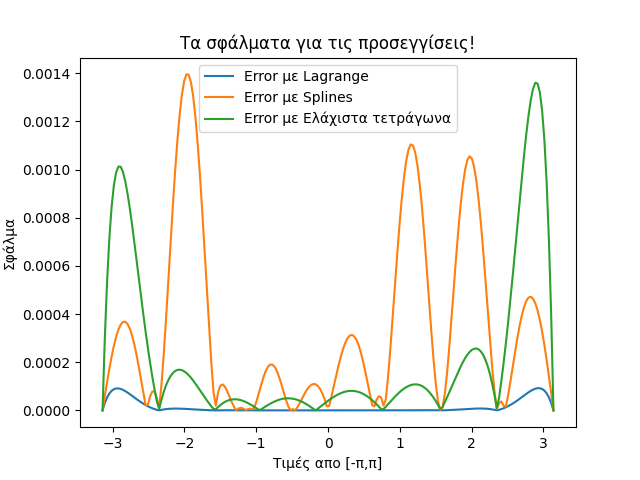
\includegraphics[width=11cm]{Errors.png}
    \end{figure}
    
    
\end{document}